% Drawing 156-8/05-1 -- folder 156-8, batch 05, archive page 92 (PDF page 93).
% Transcription: une région allongée en fuseau, hachurée, d'extrémités $0$ et $1$ ; deux bandes verticales la traversent, marquées $a$ et $b$ ; une flèche désigne un point $x$ dans la bande $b$.
% Kind: plane figure (hatched spindle with bands). Method 2 (schematic redraw from the facsimile). Status: ok.
% Notes: A spindle-shaped region from 0 to 1, lightly hatched, crossed by two vertical bands a and b (b ruled with three strokes), an arrow pointing to x in band b. The scanner's black edge crosses the bottom of the bbox.
% Coordinates: 1 unit = 1 mm = 1/100 of the crop width (bbox in page fractions: [0.33, 0.79, 0.63, 0.88]).
% Redrawn by Claude (claude-opus-5-5), issue #73 pilot, 2026-11-07; not checked by a human; not compiled (no TeX in the session).
% Rights: reproduces part of the work -- behind RENDER_TRANSCRIPTS, never published by itself.
\documentclass[tikz,border=3pt]{standalone}
\usepackage{amsmath,amssymb}
\usetikzlibrary{patterns,arrows.meta}
\tikzset{pencil/.style={black!45}, struck/.style={black!35}, mark/.style={circle,draw,inner sep=1.3pt}, pt/.style={circle,fill,inner sep=0.9pt}, opt/.style={circle,draw,fill=white,inner sep=1.1pt}}
\begin{document}
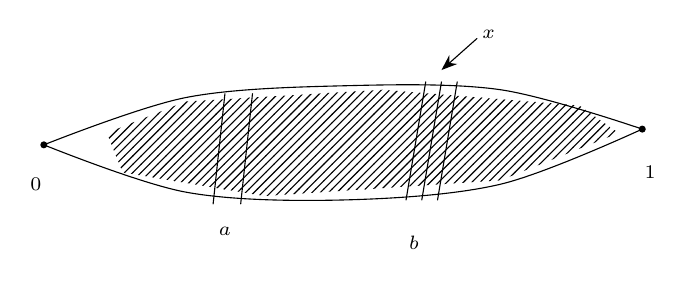
\begin{tikzpicture}[x=1mm,y=1mm,line cap=round,line join=round,font=\scriptsize]
\draw plot[smooth, tension=0.55] coordinates {(12,-20.5) (30,-14.5) (50,-13) (70,-13.5) (88,-18.5)};
\draw plot[smooth, tension=0.55] coordinates {(12,-20.5) (30,-26.5) (50,-27.5) (70,-25.5) (88,-18.5)};
\node[pt] at (12,-20.5) {};
\node[pt] at (88,-18.5) {};
\fill[pattern=north east lines] (20,-19) -- (30,-15) -- (55,-13.5) -- (80,-15.5) -- (85,-19) -- (70,-25) -- (40,-27) -- (22,-24) -- cycle;
\draw (35,-14) -- (33.5,-28);
\draw (38.5,-14) -- (37,-28);
\draw (60.5,-12.5) -- (58,-27.5);
\draw (62.5,-12.5) -- (60,-27.5);
\draw (64.5,-12.5) -- (62,-27.5);
\draw[-{Stealth[length=2mm]}] (67,-7) -- (62.5,-11);
\node[inner sep=1pt] at (68.5,-6.5) {\scriptsize $x$};
\node[inner sep=1pt] at (11,-25.5) {\scriptsize $0$};
\node[inner sep=1pt] at (89,-24) {\scriptsize $1$};
\node[inner sep=1pt] at (35,-31.5) {\scriptsize $a$};
\node[inner sep=1pt] at (59,-33) {\scriptsize $b$};
\end{tikzpicture}
\end{document}
